\titleformat{\chapter}[display]
{\normalfont\Large\bfseries}{Appendix~\Alph{chapter}}{11pt}{\Large}

\appendix
\renewcommand{\thechapter}{\Alph{chapter}}
\chapter{Vector Calculus}
\section{指标运算}
指标运算其实就是在涉及到向量, 张量求和表示时, 频繁的使用$\Sigma$会降低文章的可读性, 索性人为的\uwave{规定}去掉求和符号。
\begin{proposition}{爱因斯坦求和约定}
    只要是某一项中出现的两个相同的指标\footnote{$\bigstar$不可能在某一项中出现三个相同的指标。}, 那么就理解为对这个指标求和也就是说
    \begin{center}
        \begin{math}
            \displaystyle
            c_i = \sum_{j=1}^{3}a_{ij}b_{j} \Longleftrightarrow c_i=a_{ij}b_{j} \text{\quad} (i=1,2,3)
        \end{math}
    \end{center}
    我们称$j$为\uwave{哑指标},$i$为\uwave{自由指标}, 总的来说, 这就是一种方便使用的约定记号, 而且有时候去掉求和符号后能够是我们更加清晰地进行计算。
\end{proposition}
指标运算这个东西实际上非常微妙, 一方面它能帮助你大幅度的简化运算, 另一方面它的一些操作总是让人头晕。关于哑指标和自由指标, 你需要记住的就是哑指标只是
表示求和, 所以你可以更换字母或者对换字母, 例如:$a_ib_i=a_jb_j$, $a_{ij}b_{ji}=a_{ji}b_{ij}(i\leftrightarrow j)$, 而自由指标更像是在表示某个向量
的某一个分量, 你需要对等式两边同时去替换。
\begin{define}{符号定义}
    1.克罗内克符号(Kronecker delta)\qquad\qquad
    \begin{math}
        \centering
        \delta_{ij}=\begin{cases}
            0,& i \neq j\\
            1,& i=j
        \end{cases}
    \end{math}\\
    2.列维-奇维塔符号\footnote{$\tau$表示逆序数}(Levi-Civita symbol)\\
    \begin{center}
    \begin{math}
        \epsilon_{ijk}=\begin{cases}
            1,&\tau(ijk)\text{ is even}\\
            -1,&\tau(ijk)\text{ is odd}\\
            0,&\text{any of $i,j,k$ is equal}
        \end{cases}
    \end{math} 
    \end{center}
\end{define}    
克罗内克符号常常被用来\uwave{替换指标}, 下面的关系在简化运算时非常有用。
\begin{lequation}
    \boxed{
        \delta_{ij}a_j=a_i \qquad \qquad \delta_{ij}a_{jk}=a_{ik}
    }
\end{lequation}

也就是说一旦碰到相同的指标$\delta$会将那一项的这个指标替换为$\delta$的另一个指标, 比如上面的公式$\delta$作用为$j\leftrightarrow i$。

$\epsilon$和$delta$之间有一个十分有用的关系式:
\begin{lequation}
    \boxed{
        \epsilon_{ijk}\epsilon_{klm}=\delta_{il}\delta_{jm}-\delta_{im}\delta_{jl}
    }
\end{lequation}
\begin{thinknote}
    \textbf{几个使用求和约定表示的例子:}\\
    \begin{math}
        \displaystyle
        \bm{a}\cdot\bm{b}=a_ib_i \qquad\qquad [\bm{a}\times\bm{b}]_i=\epsilon_{ijk}a_jb_k\\
        \left(\bm{A}\bm{B}\right)_{ij}=\bm{A}_{ik}\bm{B}_{kj} \qquad\qquad \bm{A}^{T}_{ij}=\bm{A}_{ji}\\
        \left|\bm{M}\right| =\epsilon_{ijk}\bm{M}_{1i}\bm{M}_{2j}\bm{M}_{3k}\Longleftrightarrow \epsilon_{pqr}\left|\bm{M}\right|=\epsilon_{ijk}\bm{M}_{pi}\bm{M}_{qj}\bm{M}_{rk}
    \end{math}
\end{thinknote}
\section{梯度, 散度, 旋度}
\begin{define}{Gradient}
    \begin{enumerate} 
        \item  梯度可以定义为垂直于等值面的向量, 且模长等于势随等值面垂直距离的变化率
        \item  使用$df=\nabla f\cdot\bm{dr}$定义梯度($\nabla f \longleftrightarrow \bm{grad}f$)
        \item  \begin{math}
                \displaystyle
                \nabla f\overset{def}{=}\lim_{\delta V \to 0}\frac{1}{\delta V} \varoiint_{\delta S} f \bm{n}dS
                \end{math}
    \end{enumerate}
\end{define}
\begin{define}{Divergence}
    \begin{center}
        \begin{math}
        \displaystyle
        \nabla \cdot \bm{u} \overset{def}{=}\lim_{\delta V \to 0}\frac{1}{\delta V} \varoiint_{\delta S} \bm{u} \cdot \bm{n}dS
        \end{math}
    \end{center}
\end{define}
\begin{define}{curl}
    \begin{center}
        \begin{math}
        \displaystyle
        \nabla \times \bm{u} \cdot \bm{\hat{n}} \overset{def}{=}\lim_{\delta S \to 0}\frac{1}{\delta S} \oint_{\delta C} \bm{u} \cdot \bm{dr}
        \end{math}\footnote[0]{$\hat{n}$是垂直于$\delta S$面元的单位矢量, 且与曲线积分绕行方向遵循右手螺旋定则}
    \end{center}
\end{define}
在直角坐标系下, 这些量的表达式只要使用$\nabla\overset{def}{=}(\frac{\partial}{\partial x},\frac{\partial}{\partial y},\frac{\partial}{\partial z})$, 类比
为向量运算法则即可, 使用爱因斯坦求和约定可以进一步简化表达式, 并进行清晰的推演, 下面列举出来的是比较重要的矢量分析公式, 除了极个别公式, 都可以用求和约定快速
推导出来。
\begin{theorem}{一些矢量公式}
    \begin{itemize}
        \item $\nabla \cdot (\nabla f)=\nabla^2 f$\footnote[1]{也可以写为$\triangle f$定义为拉普拉斯算子}
        \item $\nabla \times (\nabla f)=0$
        \item $\nabla \cdot (\nabla \times \bm{u})=0$
        \item $\nabla \times (\nabla \times \bm{u})=\nabla(\nabla\cdot \bm{u})-\nabla^2\bm{u}$
        \item $\nabla (fg)=f\nabla g+g\nabla f$
        \item $\nabla \cdot (f\bm{u})=\nabla f \cdot \bm{u} + f\nabla\cdot \bm{u}$
        \item $\nabla \times (f\bm{u})=\nabla f \times \bm{u}+f\nabla\times\bm{u}$
        \item $\nabla \cdot (\bm{u}\times\bm{v})=(\nabla\times\bm{u})\cdot\bm{v}-(\nabla\times\bm{v})\cdot\bm{u}$
        \item $\nabla \times (\bm{u}\times\bm{v})=\bm{u}(\nabla\cdot\bm{v})+(\bm{v}\cdot\nabla)\bm{u}-(\bm{u}\cdot\nabla)\bm{v}-\bm{v}(\nabla\cdot\bm{u})$\footnote[2]{这里$\bm{u}\cdot\nabla\overset{def}{=}u_i\frac{\partial}{\partial x_i}$}
        \item $\nabla(\bm{u}\cdot\bm{v})=\bm{u}\times(\nabla\times\bm{v})+\bm{v}\times(\nabla\times\bm{u})+(\bm{u}\cdot\nabla)\bm{v}+(\bm{v}\cdot\nabla)\bm{u}$
    \end{itemize}
\end{theorem}
除了这些公式, 使用梯度、散度和旋度的相关定理可以推导出关于积分的重要公式, 在这些公式中取某些特殊情况可以得到其它实用的公式(格林公式):
\begin{theorem}{Gauss 定理}
    \begin{center}
       \begin{math}
            \displaystyle
            \iiint_V \nabla \cdot \bm{u} dV=\varoiint_S \bm{u} \cdot\bm{dS}
        \end{math} 
    \end{center}
\end{theorem}
\begin{theorem}{Stokes 定理}
    \begin{center}
        \begin{math}
            \displaystyle
            \iint_S \nabla \times \bm{u}\cdot\bm{dS}=\oint_C \bm{u}\cdot\bm{dr}
        \end{math}
    \end{center}
\end{theorem}
上面两个定理给了你一个途径, 将积分式转化为微分式, 比如Maxwell方程组的两种形式转化, 还有电解质里面的极化电荷体密度和极化强度之间的关系。
其它关于格林公式等公式的导出从略, 主要思路就是选取特殊的积分向量函数你还可以根据高斯定理结合量的守恒定律推出连续性方程:
\begin{lequation}
    \boxed{
        \frac{\partial \rho}{\partial t}+\bm{u}\cdot\nabla\rho+\rho\nabla\cdot\bm{u}=0
    }
\end{lequation}
\section{曲线坐标系}
实际上要在空间中确定点的坐标, 我们真正意义上是使用的叫做\textbf{坐标曲线}的东西来确定的。比如$u_1(x,y)=c_1$你就可以看作是一个坐标曲线, 不同的方程右边不同的常数值
也就对应了不同的曲线, 再取一个曲线簇$u_2(x,y)=c_2$, 这些曲线簇会有无限多个交点, 布满整个坐标平面, 那么我们就可以使用$(c_1,c_2)$来表示一个交点的坐标, 就是告诉你
是哪条曲线和哪条曲线相交。比如说经纬度就是这个样子, 用经线和纬线的交点来确定位置。常见的直角坐标系可以看作是$x=c_1$, $y=c_2$的特例, 这个定义也可以自然的推广到三维去, 只
是这个时候坐标曲面取代了坐标曲线, 两个坐标曲面的交点再被定义成坐标曲线。
\begin{figure}[htbp]
    \centering
    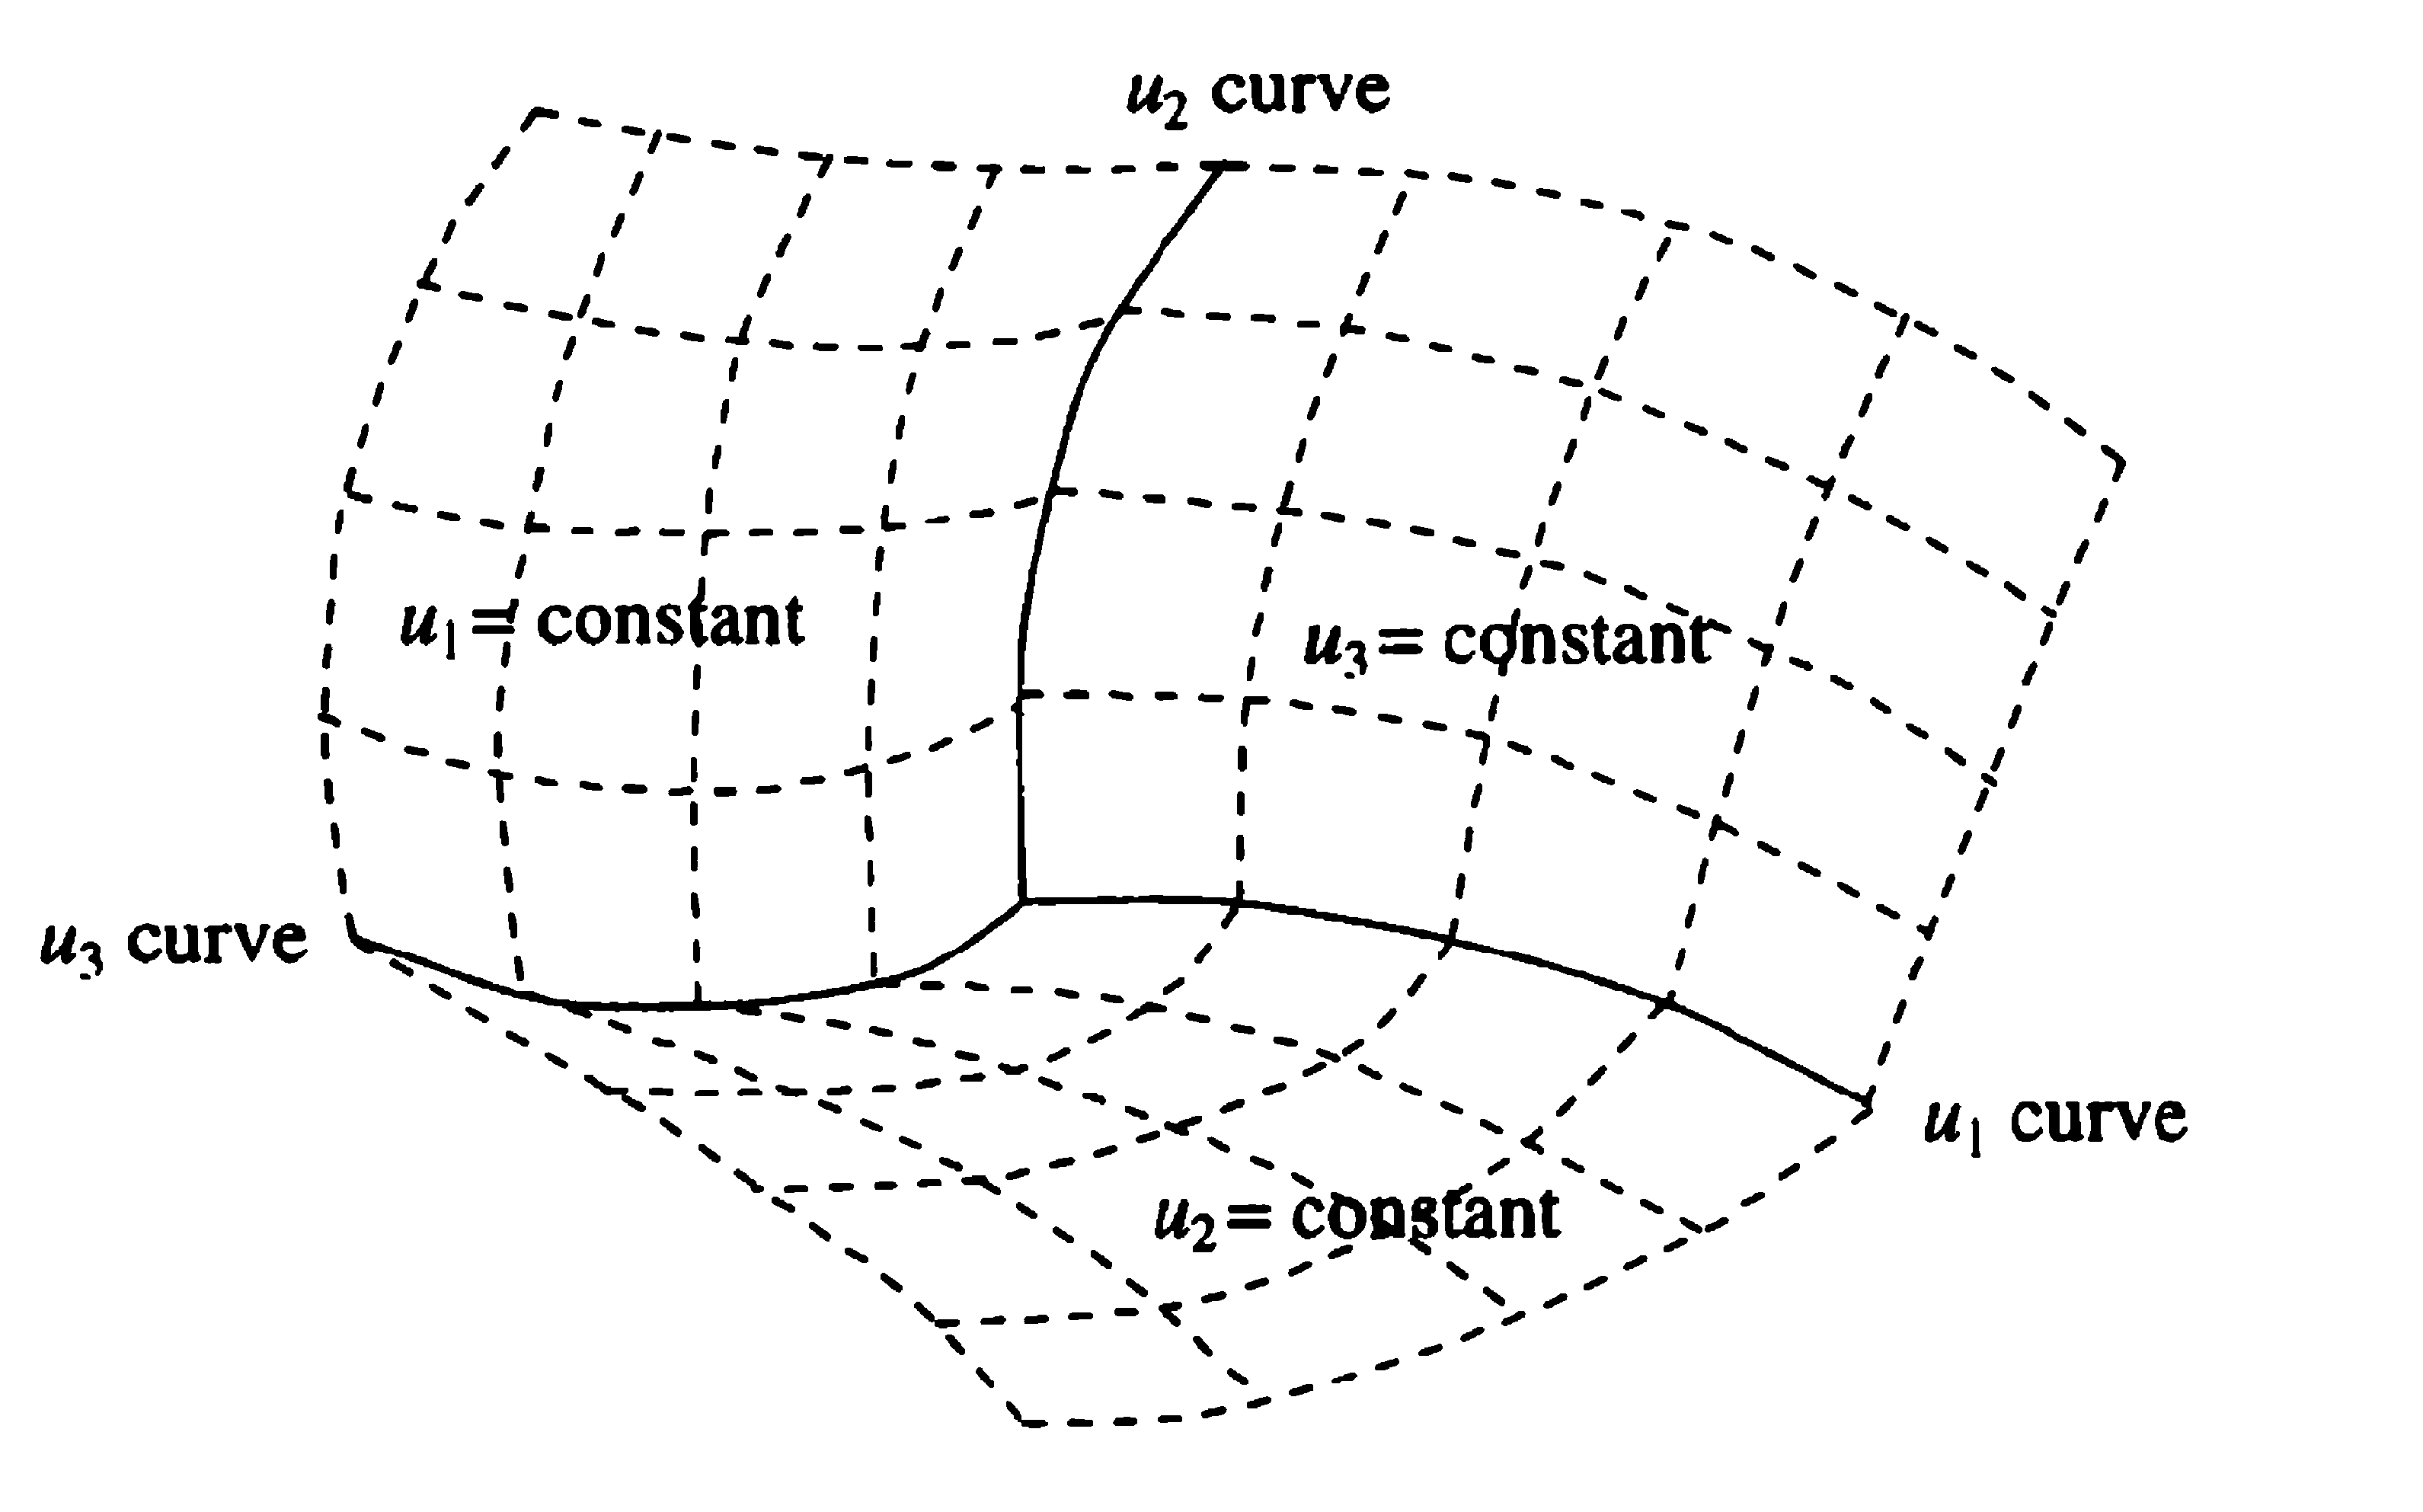
\includegraphics[scale=0.26]{fig/a-1.eps}
    \caption{曲线坐标系}
\end{figure}

特别的, 如果空间中每一个交点处坐标曲线的切线两两垂直, 那么我们称为\textbf{正交曲线坐标系}, 我们后面对于曲线坐标系中的梯度、旋度和散度的表达都是值正交曲线
坐标系的, 常见的诸如极坐标系, 球坐标系和柱坐标系都属于正交曲线坐标系。

现在我们要去看看曲线坐标系里面的微分和直角坐标系之间的关系, 我们总是倾向于去讨论局部的特征, 而且那些梯度散度的定义也是在一个无穷小下定义的。下面的讨论中, 我
们都假设坐标曲面为$$u_1(x_1,x_2,x_3)=u_1,u_2(x_1,x_2,x_3)=u_2,u_3(x_1,x_2,x_3)=u_3$$相应的, 每一点的坐标可以写成$(u_1,u_2,u_3)$。

现在我们假设直角坐标系中有一个微小的位移$\bm{dx}=(dx_1,dx_2,dx_3)$, 注意, 我们谈论两个坐标系, 他们之间一定是同坯的, 也就是说一定对应一个曲线坐标到直线坐标的
变换$$x_1(u_1,u_2,u_3)=0,x_2(u_1,u_2,u_3)=0,x_3(u_1,u_2,u_3)=0$$这样我们便可以把位移矢量使用曲线坐标系的坐标变换微元表示为:
$$dx_i=\frac{\partial x_i}{\partial u_j}du_j,\bm{dx}=\frac{\partial \bm{x}}{\partial u_j}du_j$$注意到上式我们使用了爱因斯坦求和约定。
观察每个$du_j$前面的系数$\frac{\partial \bm{x}}{\partial u_j}$, 这是一个向量, 而且是沿着关于$u_j$的这条坐标曲线的一个切向向量。很自然的, 模仿直角坐标系, 我
们引入方向向量
\begin{define}{方向向量和拉梅系数}
    \begin{lequation}
    \boxed{
        \bm{e_j}\overset{def}{=}\frac{1}{h_j}\frac{\partial \bm{x}}{\partial u_j},h_j=\left|\frac{\partial \bm{x}}{\partial u_j} \right|
    }
\end{lequation}
\end{define}
上式中的$h_j$称为\textbf{拉梅系数}, 它定义了坐标系在局部如何伸缩, 这里要明确, $du_j$只是表示坐标的变化, 虽然在通常的欧几里得空间直角坐标系中, $dx$的变化
有明确的几何意义, 它可以直接表示位移在$x$轴方向上的投影, 但是, $du$只是一个参量的变化, 没有明确的几何意义, 拉梅系数就是一种伸缩效应, 直角坐标到曲线坐标的过程中
还有伸缩, 拉梅系数就决定了这种伸缩的大小, 决定了你坐标参量变化与实际在$u_j$的方向产生的长度变化的比例关系。
\begin{thinknote}
    这里还要说明一点, 拉梅系数和单位矢量的方向、大小
    在每一点一般都是\textbf{不同的}!, 这也就是曲线坐标系让人头疼的地方, 比如你要使用曲线坐标的导数表示速度, 你需要考虑单位矢量随着质点移动的变化, 你需要对单位矢量求导!
    (实际上方向导数不是随时间变化的, 只是每一点的方向导数不同, 而质点的坐标又随时间变化)。这恰恰也就是为何极坐标系下速度的导出式子相对麻烦。
\end{thinknote}
在正交曲线坐标系中还有下面的正交关系:$$\bm{e_i}\bm{e_j}=\delta_{ij}$$
\begin{theorem}{曲线坐标系下的微元}
    \begin{itemize}
        \item $\bm{dx}=h_1\bm{e_1}du_1+h_2\bm{e_2}du_2+h_3\bm{e_3}du_3$
        \item $dS_1=h_2h_3du_2du_3$
        \item $dV=h_1h_2h_3du_1du_2du_3$
    \end{itemize}
\end{theorem}
上式中$dS$和$dV$就是指以坐标曲面/曲线去分割整个空间得到的面积微元和体积微元。也就是常常我们使用坐标变换求体积分或者是面积分要做的第一件事情, 求微元, 而且由于我们
使用的求积分的方法, 要求的微元一定是要按照坐标曲线去分割的。这里你要是使用Jacobi行列式去求, 结果相同, 实际上$J=\frac{\partial \bm{x}}{\partial u_1}\cdot
\frac{\partial \bm{x}}{\partial u_2}\times\frac{\partial \bm{x}}{\partial u_3}$, Jacobi行列式的实质是这三个向量的混合积。我认为使用这个方法更能体现出几何实质(\ref{曲线坐标微元})。
按照坐标曲线去划分出微元然后再使用梯度、旋度和散度的定义(梯度使用定义式$df=\nabla f \cdot \bm{ds}$), 可以很容易地推出下面的式子:
\begin{theorem}{梯度、旋度和散度在曲线坐标系下的表现形式}
    \begin{itemize}
        \item $\nabla f = \frac{1}{h_1}\frac{\partial f}{\partial u_1}\bm{e_1}+\frac{1}{h_2}\frac{\partial f}{\partial u_2}\bm{e_2}+\frac{1}{h_3}\frac{\partial f}{\partial u_3}\bm{e_3}$
        \item $\nabla \cdot \bm{v} = \frac{1}{h_1h_2h_3}\left(\frac{\partial}{\partial u_1}(v_1h_2h_3)+\frac{\partial}{\partial u_2}(v_2h_3h_1)+\frac{\partial}{\partial u_3}(v_3h_1h_2)\right)$
        \item $\nabla^2 f = \frac{1}{h_1h_2h_3}\left[\frac{\partial}{\partial u_1}\left(\frac{h_2h_3}{h_1}\frac{\partial f}{\partial u_1}\right)\right]
               +\frac{\partial}{\partial u_2}\left(\frac{h_3h_1}{h_2}\frac{\partial f}{\partial u_2}\right)
               \frac{\partial}{\partial u_3}\left(\frac{h_1h_2}{h_3}\frac{\partial f}{\partial u_3}\right)$
        \item 
        \begin{math}
            \displaystyle
            \frac{1}{h_1h_2h_3} 
            \begin{vmatrix}
            h_1\bm{e_1}&  h_1\bm{e_2} & h_1\bm{e_2} \\
            \frac{\partial }{\partial u_1} & \frac{\partial }{\partial u_2} & \frac{\partial }{\partial u_3}\\
            h_1v_1 & h_2v_2 & h_3v_3
            \end{vmatrix}
        \end{math}
    \end{itemize}
\end{theorem}
\begin{thinknote}
    下面来推导一下最后一个式子:
    $$\nabla \times \bm{u} \cdot \bm{\hat{n}} \overset{def}{=}\lim_{\delta S \to 0}\frac{1}{\delta S} \oint_{\delta C} \bm{u} \cdot \bm{dr}$$

    考虑一个在$u_3$坐标曲面上的小矩形(\ref{旋度计算}), 也即$u_1$和$u_2$变化时产生的几何微元, 利用这个矩形去求旋度在$e_3$方向上的分量大小。

    首先计算环量, 注意到$\bm{v}$的分量的方向以及积分方向的关系, 不难得到左右两边积分为
    $$[v_2h_2](u_1+\frac{du_1}{2},u_2,u_3)du_2-[v_2h_2](u_1-\frac{du_1}{2},u_2,u_3))du_2$$
    注意, 这里$v_2h_2$是随着坐标而变化的, 将$v_2h_2$整体看成是一个函数, 只有$u_1$变了, 泰勒展开进行一阶近似得到
    $$\frac{1}{h_1h_2}\frac{\partial}{\partial u_1}(v_2h_2)$$
    类似的方法可以计算出上下边的积分为:
    $$-\frac{1}{h_1h_2}\frac{\partial}{\partial u_2}(v_1h_1)$$
    注意到我们这样计算最后得到的是垂直于积分曲线围成的曲面的法向方向旋度分量, 也即:
    $$\bm{e_3}\cdot\nabla\times\bm{v}=\frac{1}{h_1h_2}\left(\frac{\partial}{\partial u_1}(v_2h_2)-\frac{\partial}{\partial u_2}(v_1h_1)\right)$$
    对每一个方向都进行计算后便可以得到上面的公式
\end{thinknote}
物理量比如速度表达式的推导只需要将时间$t$这个参数引入就行了。比如:$$\bm{v}=\frac{\bm{dx}}{dt}=h_1\dot{u_1}\bm{e_1}+h_2\dot{u_2}\bm{e_2}+h_3\dot{u_3}\bm{e_3}$$
要求加速度, 将上式对时间再求一阶导数即可。在这里重新说明一下, 这个单位矢量本身不是随时间变化的, 是随空间坐标变化的, 但是质点运动时, 空间坐标显含时间, 所以相当于是
质点自身来看, 单位矢量隐含时间项。
\begin{figure}[htbp]
    \centering
    \label{旋度计算}
    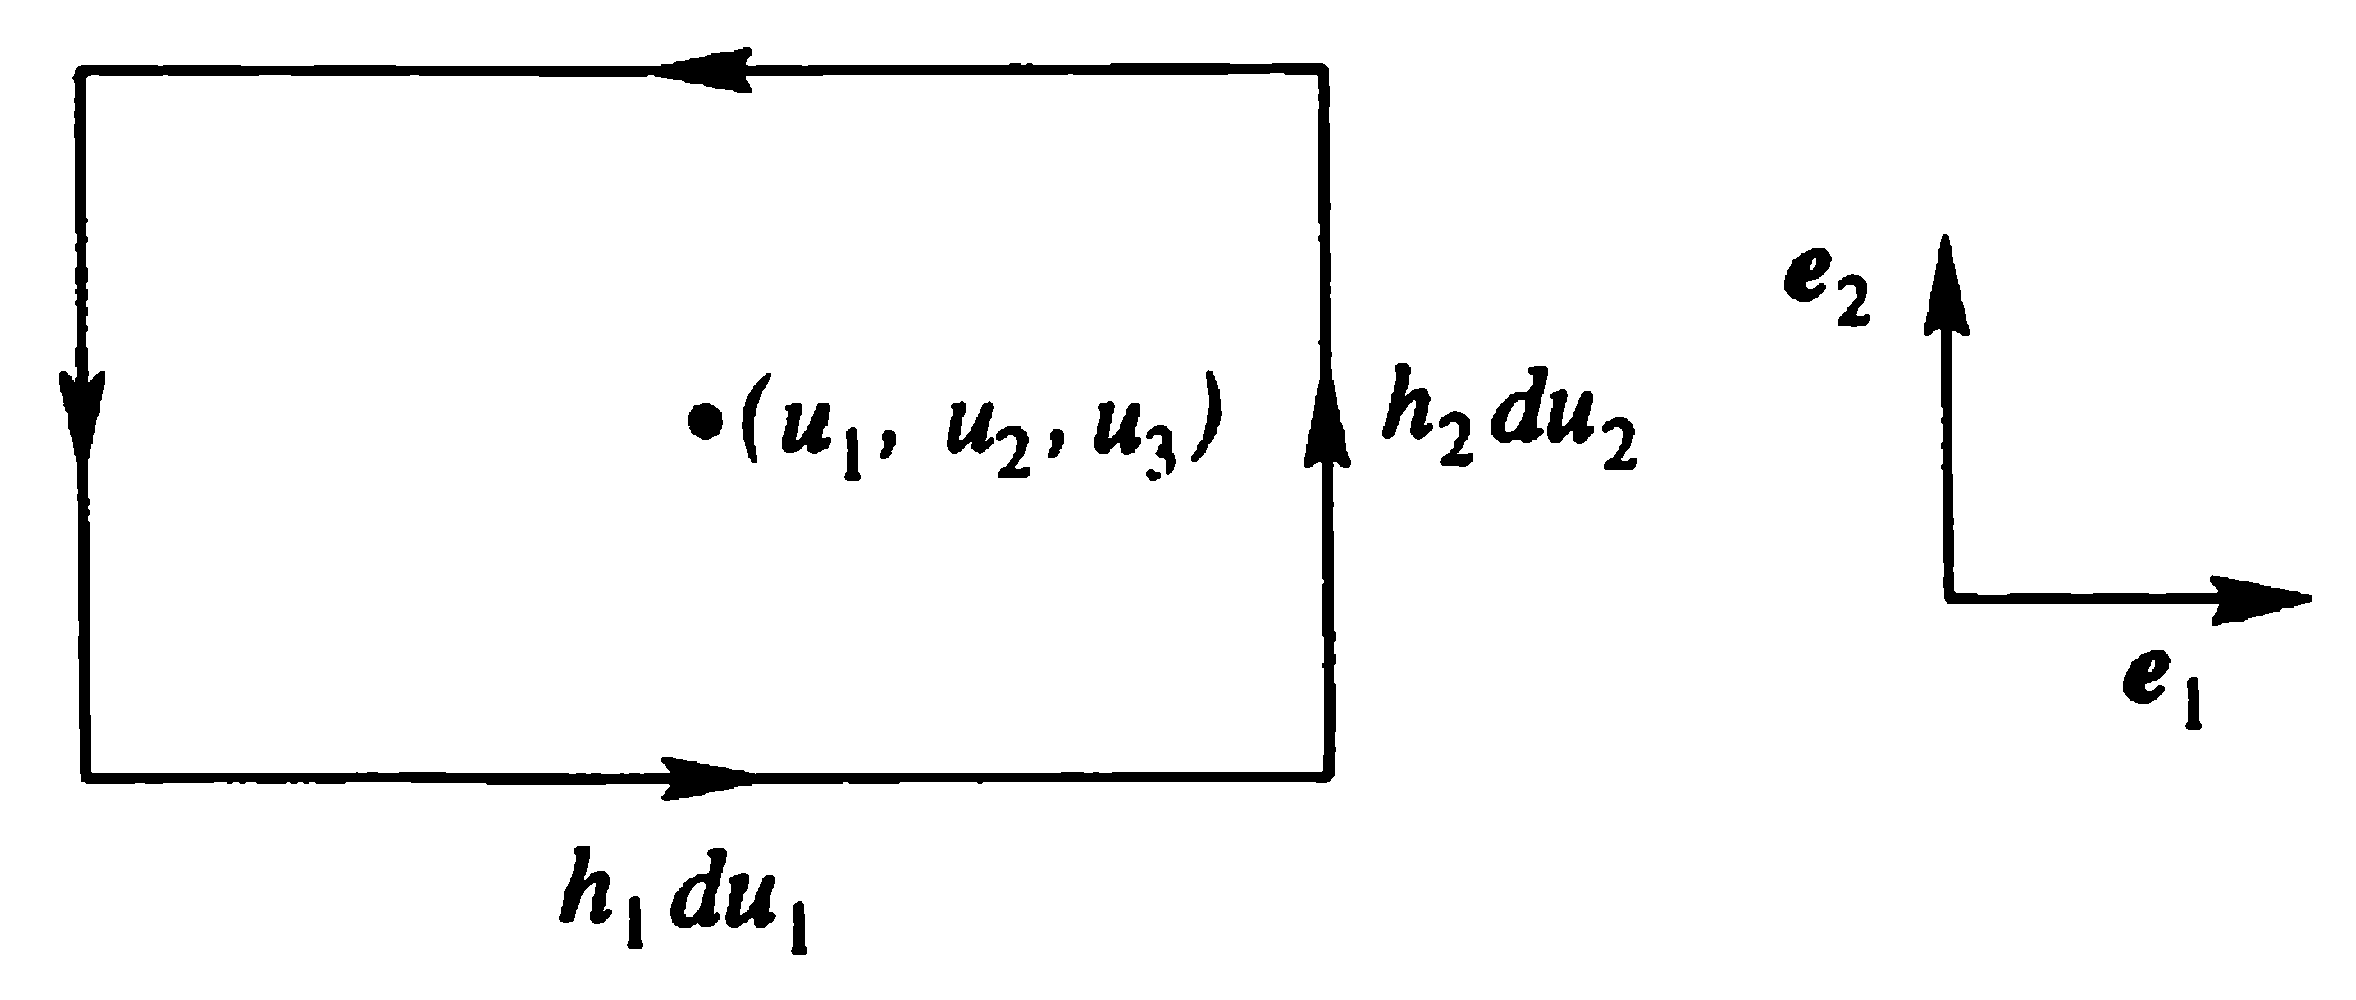
\includegraphics[scale=0.3]{fig/a-3.eps}
    \caption{计算旋度}
\end{figure}
\begin{figure}[htbp]
    \centering
    \label{曲线坐标微元}
    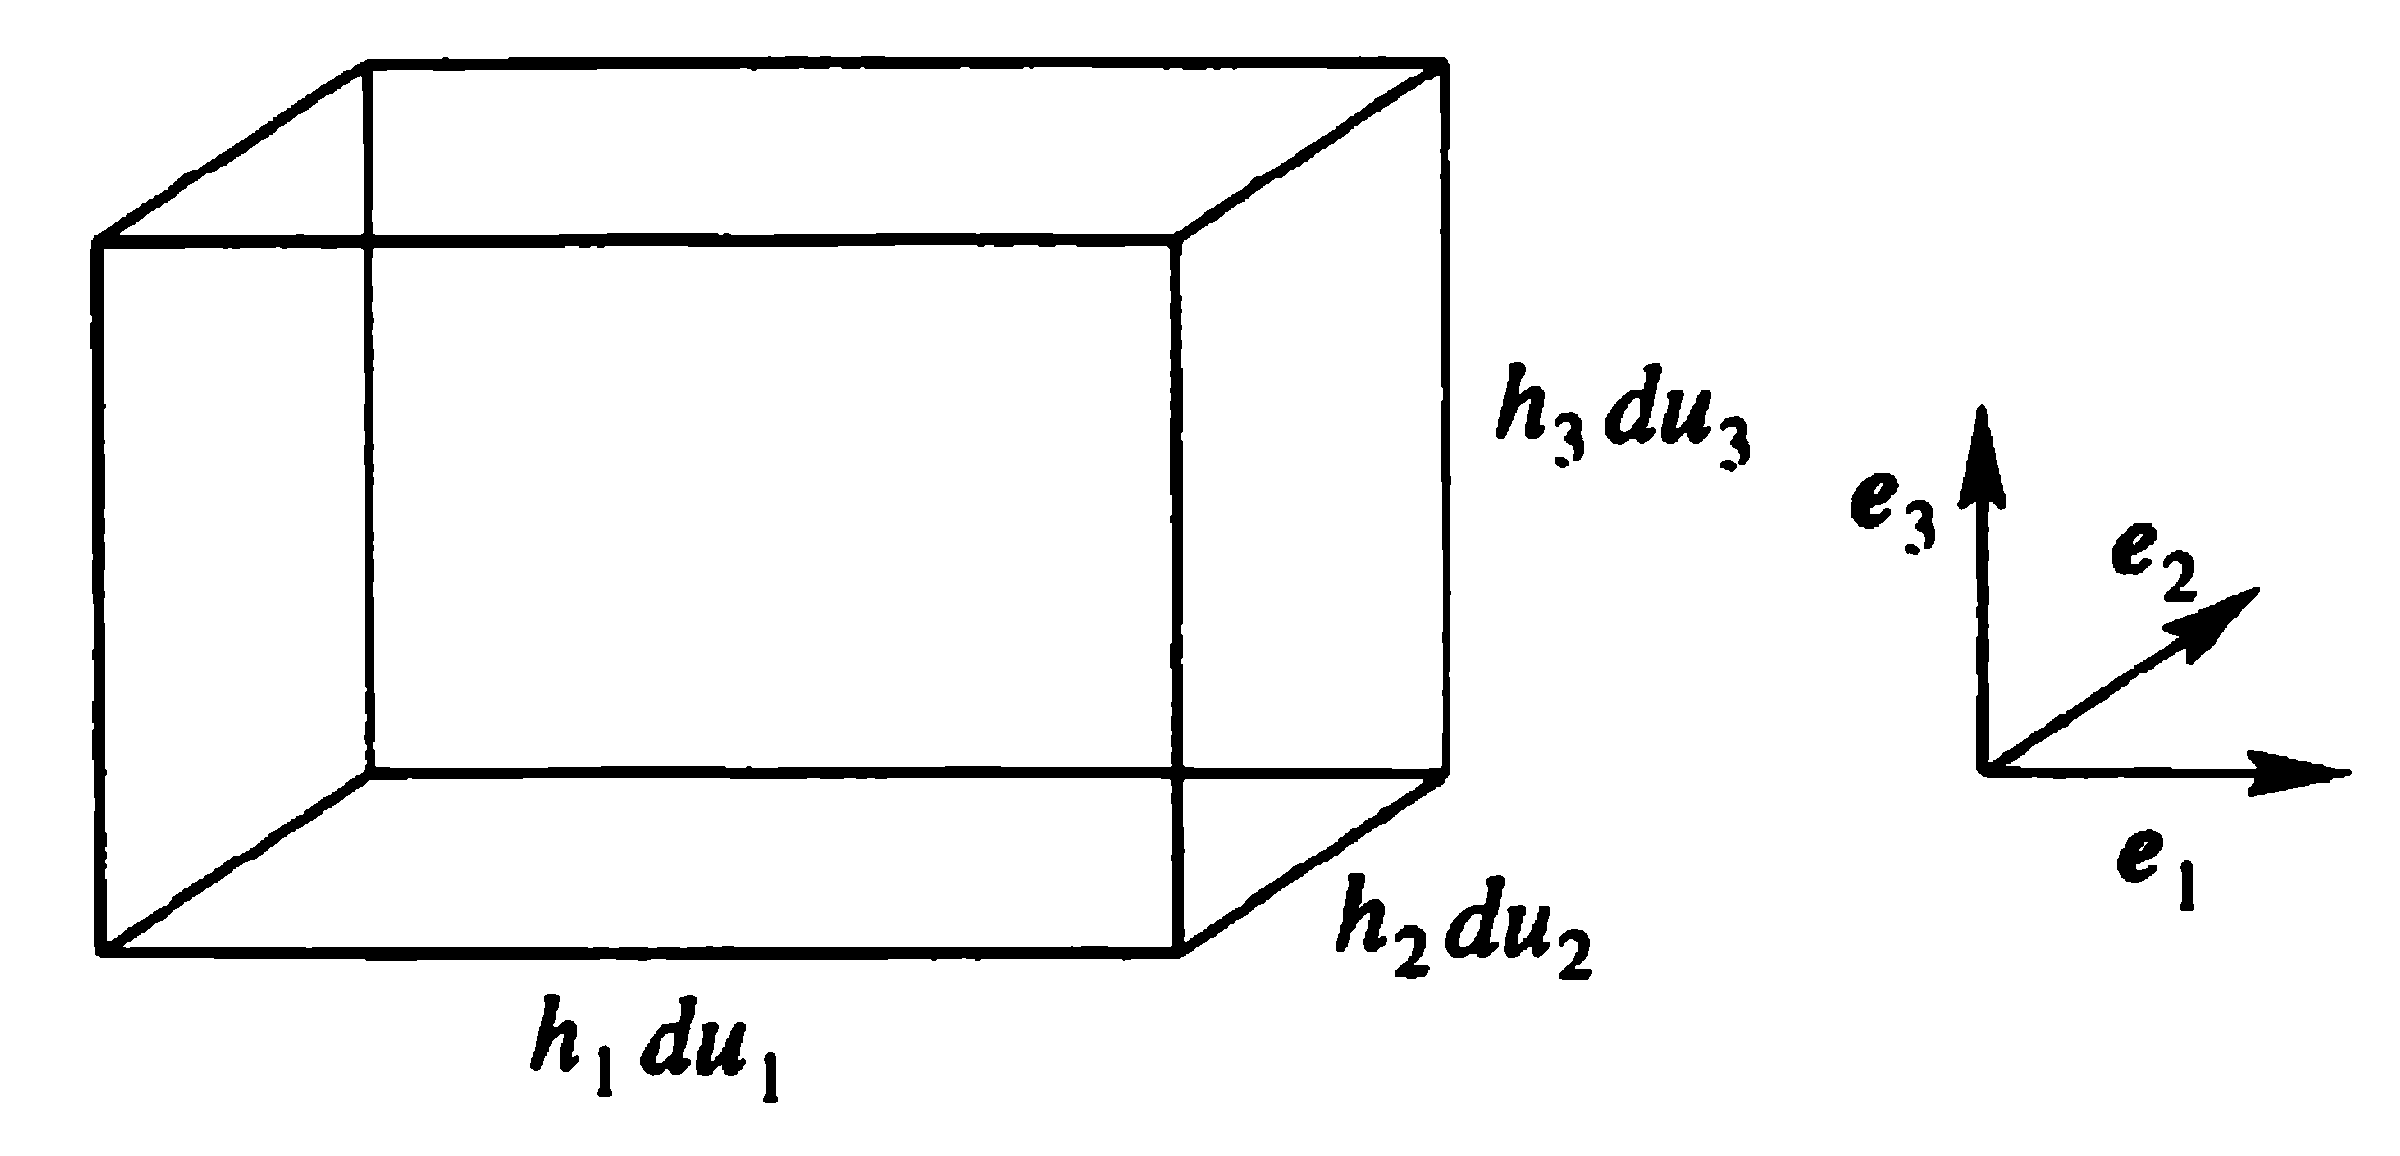
\includegraphics[scale=0.26]{fig/a-2.eps}
    \caption{曲线坐标系的局部就可以看成一个小(不再是直角坐标里面的正方体了), 图中也标出了参数微元和实际位移量的比例关系}
\end{figure}
\section{直角坐标里的张量}
在探讨什么是张量之前, 我们需要重新定义一下什么是标量和矢量, 下面的讨论都是在直角坐标系下的。

考虑坐标系的旋转, 空间中某一点在两个坐标系中的坐标$\bm{X'}$和$\bm{X}$由一个过渡矩阵$\bm{L}$联系起来。这个矩阵就是我们所熟知的\uwave{转动矩阵}, 是一个正交
矩阵
\begin{lequation}
    \boxed{
        \bm{L}=
        \begin{pmatrix}
           \cos\theta & \sin\theta \\
           -\sin\theta& \cos\theta
        \end{pmatrix}
    }
\end{lequation}
\begin{center}
    \begin{math}
        \displaystyle
        \begin{pmatrix}
            x_1' \\
            x_2'
        \end{pmatrix}
        =\bm{L}
        \begin{pmatrix}
            x_1\\
            x_2
        \end{pmatrix}
        \qquad
        \bm{L}\bm{L^T}=\bm{L^T}\bm{L}=\bm{I}
        \qquad
        \left|\bm{L}\right|=1
    \end{math}
\end{center}
上面的后两个式子是正交矩阵自身的性质, 第一式使用求和约定写成
\begin{center}
    \begin{math}
        \displaystyle
        x_i'=L_{ij}x_j\qquad
        x_i =L_{ji}x_j'
    \end{math}
\end{center}
注意用到了$\bm{L^T}=\bm{L^{-1}}$这个条件。对于更高纬度的欧式空间, 每个基向量若还是有正交关系, 即$\bm{e_i}\cdot\bm{e_j}=\delta_{ij}$。旋转变换是保长
变换, 我们仍旧可以使用两个坐标基向量之间的确定转换矩阵为
\begin{lequation}
    \boxed{
        L_{ij}=\bm{e_i'}\cdot\bm{e_j}
    }
\end{lequation}
这个矩阵还是一个正交矩阵, 但是注意, $L^TL=I$不能说明$\left|L\right|=\pm 1$, 行列式的值取$1$才表示\textbf{旋转变换}, 取$-1$表示\textbf{反射变换}。
这个矩阵还是一个实矩阵, 是一个\uwave{等距同构}算子的矩阵, 线性代数中可以证明实内积空间上的等距同构\footnote[1]{回忆一下等距同构一定是正规的}的矩阵有下面性质
\begin{theorem}{实内积空间上的等距同构}
    如果$S$是实内积空间上的某个等距同构, 那么它关于某个规范正交基的矩阵一定是一个分块对角阵, 而且每个块中的元素是$\pm 1$或者
    \begin{center}
        \begin{math}
            \displaystyle
            \begin{pmatrix}
                \cos\theta & \sin\theta \\
                -\sin\theta& \cos\theta
            \end{pmatrix}
        \end{math}
    \end{center}
\end{theorem}
显然, 我们这里的等距同构就是一个$R^n$上的旋转变换, $L$就是它的矩阵表示。下面还有关于$L$的两个等式:
\begin{lequation}
    \frac{\partial x_i'}{\partial x_j}=L_{ij} \qquad \text{and} \qquad \frac{\partial x_i}{\partial x_j'}=L_{ji}
\end{lequation}
\begin{define}{标量和矢量}
    \begin{itemize}
        \item 
        $\bm{v}$是一个矢量, 当且仅当在坐标系进行旋转变换时, 它在两个坐标系下的分量之间的变换与$\bm{L_{ij}}$一致, 也就是说它的变换和点的变换时一致的:$$v_i'=L_{ij}v_j$$
        \item 标量定义为在坐标系的旋转变换下,值始终不变的量$$s'=s$$
    \end{itemize}
\end{define}
我们抛弃了原先矢量的定义, 一个有大小有方向的量, 取而代之的是一个更加抽象化的描述, 也更加精确, 同时也为我们将定义扩展到张量上带来了便利, 使用定义我们可以证明
两个矢量的点乘是标量。
\begin{thinknote}
    对于矢量$\bm{a}$和$\bm{b}$我们有$$a_i'=L_{ij}a_j,b_i'=L{ij}b_j$$那么$s=\bm{a}\cdot\bm{b}=a_ib_i$, 换到另一个参考系后, 点乘的定义还是不变有
    \begin{center}
        \begin{math}
            s'=(\bm{a}\cdot\bm{b})'=a_i'b_i'=L_{ij}a_jL_{ik}b_k=L_{ij}L_{ik}a_jb_k=\delta_{jk}a_jb_k=a_kb_k=s
        \end{math}
    \end{center}
    这就证明了$\bm{a}\cdot\bm{b}$是标量。 
\end{thinknote}
这也是证明一个量是否是矢量或标量的一般方法
\footnote[1]{注意到上面的证明利用了
    $$\bm{L}\bm{L^T}=\bm{I}\Rightarrow L_{ij}L^T_{jk}=\delta_{ik} \xLongrightarrow{L^T_{jk}=L_{kj}} L_{ij}L_{kj}=\delta_{ik}$$
    使用$\bm{L^T}\bm{L}=\bm{I}$可以导出我们证明需要的等式}
, 考虑它的基本得到方法, 然后再两个坐标系下的表示, 最后考虑其分量随
坐标变换的变换关系。

下面将定义推广到张量, 我们前面接触的矢量, 只有一个自由指标, 但是张量却有多个自由指标。
\begin{define}{张量}
    $T$是一个\uwave{二阶张量}, iff.坐标变换时满足$$T'_{ij}=L_{ik}L_{jm}T_{km}$$同理, 三阶张量就是坐标变换时满足下面关系的量$$P'_{ijk}=L_{ip}L_{jq}L_{kr}P_{pqr}$$
    我们也常常将标量称为\uwave{零阶张量}, 矢量称为\uwave{一阶张量}。
\end{define}
前面提到的$\delta_{ij},\epsilon_{ijk}$就是张量的例子, 证明方法和证明一个量是否是矢量类似, 下面介绍一个很有用的定理去判断一个量是不是张量, 在物理定律中可以用
它来迅速发现一个量的张量本质。
\begin{theorem}{商法则(Quotient Rule)}
    $$a_i=T_{ij}b_j$$
    如果对于坐标系的任何一个变换, 对于任何一个矢量$\bm{b}$, 使用上面式子计算出来的$\bm{a}$都是一个矢量, 那么$T$是一个张量。
    
    这个定理还可以推广, 如果对于任意一个$n$阶张量$B$和任意坐标变换使用下面的式子得到的$A$总是个$m$阶张量, 那么$T$一定是一个$m+n$阶张量。
    \begin{center}
        \begin{math}
            \displaystyle
            A_{\underbrace{ijk\ldots}_{m}}=T_{\underbrace{ijk\ldots\alpha\beta\gamma\ldots}_{m+n}}B_{\underbrace{\alpha\beta\gamma\ldots}_{n}}
        \end{math}
    \end{center}
\end{theorem}
直角坐标系里, 我们可以使用一个n-by-1的矩阵表示一个向量, 而对于一个二阶张量我们需要一个二维的n-by-n矩阵去描述, 三阶张量需要使用一个立体的矩阵去描述, 到了
更高维就很难去想象这样一个“矩阵”了。注意, 张量、矢量本身是不随坐标系变换改变的, 只是分量在不同坐标系下可能不同, 所以不同坐标系下描述它的矩阵可能有点差别。

\begin{define}{对称张量和反对称张量}
    这个的定义和对称矩阵的定义非常相似 
    \begin{itemize}
        \item \textbf{对称张量}: 任意两个下标对换后得到的两个分量始终相等, 如$T_{ij}\equiv T_{ji}$
        \item \textbf{反对称张量}: 任意两个下标对换后得到的两个分量始终互为相反数, 如$T_{ij}\equiv -T_{ji}$
    \end{itemize}
    $\delta_{ij}$是对称张量, $\epsilon_{ijk}$是反对称张量, 所以$ijk$中任何两个值相等时$\epsilon=0$。

    虽然不同的坐标系下张量的分量不同, 但张量对称性质不随坐标系的变换而变化。
\end{define}
\begin{define}{各向同性张量}
    如果一个张量的每一个分量在不同的坐标系下都相同, 那么这个张量称为\textbf{各向同性张量}。
\end{define}
各向同性张量事实上非常少可以证明各向同性张量只可能是下面的形式:
\begin{proposition}{n阶各向同性张量}
    \begin{itemize}
        \item 0-order: 都是各向同性的
        \item 1-order: 只有$\bm{0}$是各向同性的
        \item 2-order: 只有$a_{ij}=\lambda \delta_{ij}$是各向同性的
        \item 3-order: 只有$a_{ijk}=\lambda \epsilon_{ijk}$是各向同性的
        \item 4-order: 只有$a_{ijkl}=\lambda\delta_{ij}\delta_{kl}+\mu\delta_{ik}\delta_{jl}+\nu\delta_{il}\delta_{jk}$是各向同性的
    \end{itemize}
\end{proposition}
在物理学中, 张量的出现总是伴随着两个矢量, 使用商法则, 我们就可以判断一个量是张量, 正是张量的存在才让两个矢量之间的关系变得复杂起来。
\subsubsection*{电导率张量}
我们先回顾一下欧姆定律的微分形式$$\bm{j}=\sigma\bm{E}$$初学电磁学时会简单的认为$\bm{j}$和$\bm{E}$的方向相同, 只是在所谓的长度上有一个伸缩关系。实则不然
在一般的介质中, 这两个矢量是不平行的, 我们考虑一个极端情况
\begin{figure}[htbp]
    \centering
    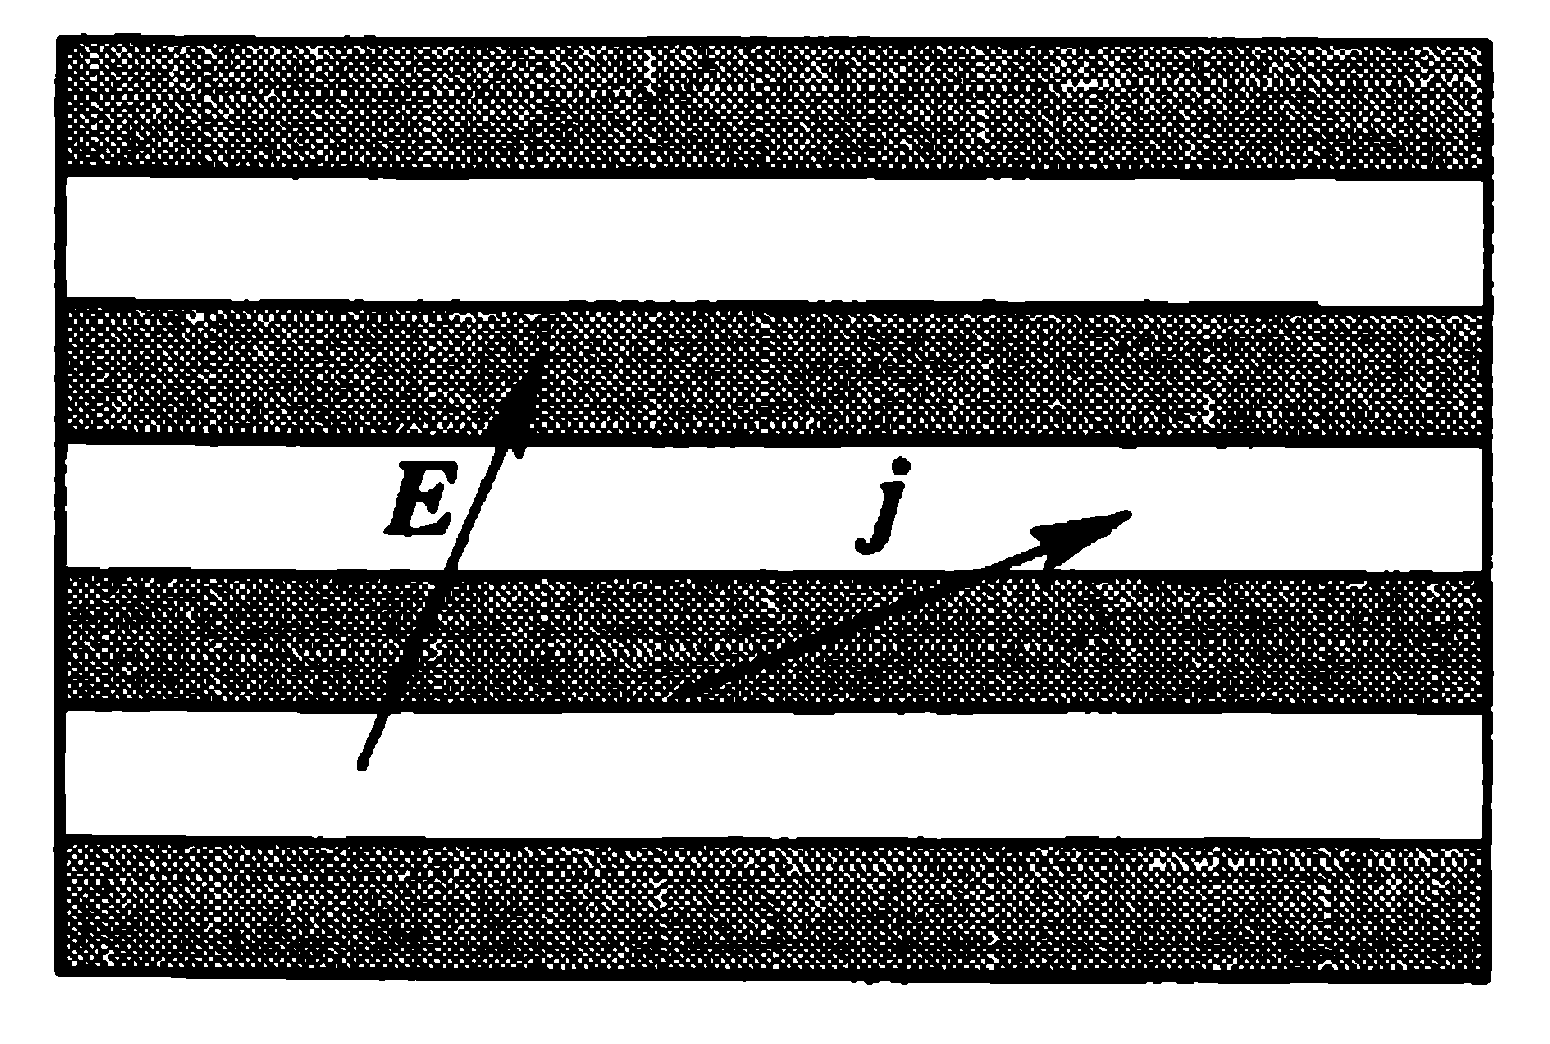
\includegraphics[scale=0.3]{fig/a-4.eps}
    \caption{电导率张量}
\end{figure}
这个介质是由两种不同的介质构成的,不再和我们一般的介质一样是各向同性的, 在每一层介质中, 和我们之前学的确实是一致的, 但是当你考虑边界面处$\bm{j}$和$\bm{E}$的
关系时, 会有很大的不同。 我们假设白色的介质电导率很低,就像是绝缘体一样, 而灰色的介质导电率很高, 是一个良导体。这个时候显然电流更容易沿着边界面流动, 而不是
穿过界面\footnote[1]{你可以想象一堵墙阻挡你, 无论别人用多大的力气推你, 你也只能沿着墙走},所以就会导致两个矢量方向不同, 这个时候如果$\sigma$是一个标量肯定
不符合要求, 这个时候就要求$\sigma$是一个张量了, 而且$$j_i=\sigma_{ik}E_k$$在我们讨论的这个情况下, 这个张量可以使用矩阵描述为:
\begin{center}
    \begin{math}
        \displaystyle
        \sigma=
        \begin{pmatrix}
            \sigma_0&0&0\\
            0&\sigma_0&0\\
            0&0&0
        \end{pmatrix}
    \end{math}
\end{center}
其中$x$轴平行于分界面, $y$轴垂直于分界面, $z$轴垂直于纸面。

当我们讨论的介质各向同性, 每个地方的电导率相等时, 这个张量和我们前面定义的各向同性张量是一样的, 分量不随坐标系变换而变化。那么$\sigma_{ij}=\sigma_0\delta_{ij}$
$$j_i=\sigma_{ik}E_k=\sigma_0\delta_{ik}E_k=\sigma E_i\Rightarrow\bm{j}=\sigma_0bm{E}$$张量退化为了我们熟知的标量。
\subsubsection*{惯量张量}
初学力学时, 一直在强调, 刚体的角动量和角速度一般情况下方向是不同的, 我们刚体平行平面运动中所列的转动方程实际上是列的投影式$M_z=I_{zz}\frac{d\omega_z}{dt}$(其中转轴就是
$z$轴, 角速度方向和$z$轴方向相同), 这也说明转动惯量也应该是一个张量, 只是我们在计算的都是均匀的几何体, 具有各向同性, 惯量张量退化为一个标量。惯量张量也可以
表示为一个矩阵, 对角线元素是转动惯量, 非对角线元素叫做惯量积。Feynman讲义第一卷中也讨论了这个问题, 就是因为几何体的不均匀性才导致了转动惯量是张量, 这一点
在刚体做定轴转动是尤为明显。

我们下面计算一个刚体绕某个基点以$\Omega$角速度转动时的角动量矢量的第$i$个分量:
\begin{center}
    \begin{equation*}
        \displaystyle
        \begin{split}
            L_i&=\iiint_V \rho(\bm{r}\times\bm{v})_idV\\
               &=\iiint_V \rho(\bm{r}\times\left(\bm{\Omega}\times\bm{r}\right))_idV\\
               &=\iiint_V \rho\left(r^2\Omega_i-\left(\bm{r}\cdot\bm{\Omega}\right)r_i\right)dV \qquad\qquad\text{(Lagrange恒等式)}\\
               &=\iiint_V \rho\left(r^2\delta_{ij}\Omega_j-r_j\Omega_jr_i\right)dV\\
               &=\iiint_V \rho\left(r^2\delta_{ij}-r_jr_i\right)\Omega_jdV\\
        \end{split}
    \end{equation*}
\end{center}    
定义惯量张量$$I_{ij}=\iiint_V \rho\left(r^2\delta_{ij}-r_jr_i\right)$$
那么角动量和角速度之间的关系又下式给定:
$$L_i=I_{ij}\Omega_j$$
再从角速度和角动量的矢量性质, 由商法则可以判断$I$是二阶张量, 也正是由于它的张量性质才有了角动量和角速度方向的不同。



\chapter{Linear Algebra}


\chapter{Gaussian Integral}